%lost on page 11 - extracted and used climate variables
%cartoon of whole procedure for climate variables
%figure showing correlation b/t bio12 and 
%state that VSURF importance is different scales in different models
%moved up three hypotheses part to introduction
%play up lack of GxE and ???
%** correct # of Pop x Treatment
% model of growth chamber
% need to explain 'importance'

%* delve into interactions - do they change cline?

%* show figures of reaction norms
%* split plot, account for error variation in temp???
%* show PAR similarity
%* some sites they are functionally annual

%* hung up on specialization - clarify? where is ecological oppportunity, tradeoffs, specialization
%	- maybe temporal source-sink makes more sense

%* explain rhizomes

%* put in biomass allocation cline
% TO DO:
% 1. Is water regime on figure 1 correct? (data is in office)
% 2. Double check spatially averaged analysis
% 3. For Figure_PC1vLat: plot axes could be range maps with areas highlighted (x-axis) and short to tall plants (y-axis)
% 4. Do anything with biomass data? Currently, NO.

% 5. Citations for latitudinal clines
	% cases where clinal variation has 'obvious' selective source:
	% Antonovics and Bradshaw discuss steepness of clines and strength of selection over 10's of meters off mines in Anthoxanthum
	% Caicedo et al 2004?
	% clines in phenotypic traits reviewed by Hedrick 2006, Schemske and Bier 2007
% 6. Citations for GxE as signature of local adaptation

\documentclass[11pt, oneside]{article}

%
% Packages
%

\usepackage{geometry}
\geometry{letterpaper}
\usepackage[parfill]{parskip}      		% Activate to begin paragraphs with an empty line rather than an indent
\usepackage{graphicx}
\usepackage{booktabs}
\usepackage{topcapt}
\usepackage[labelfont =  {sf, bf}, textfont = sf, format = plain]{caption}
\usepackage{amssymb}
\usepackage{amsmath}
\usepackage{natbib}
\usepackage{color}
\usepackage{array}
\usepackage{gensymb}
\usepackage{setspace}
\newcommand{\stretchy}{1.5}
\usepackage{lineno}
\usepackage{textcomp}

% Make helvetica the default sans-serif font
% \renewcommand\sfdefault{phv}

% Package command for citing R packages
\newcommand{\pkg}[1]{{\fontseries{b}\selectfont #1}} 

%
% Commenting
%

\newcommand{\cdm}[1]{{ \color{magenta} [{\bf{CDM:}} {\em#1}]}} % Chris' comments are in magenta.
\newcommand{\ala}[1]{{ \color{blue} [{\bf{ALA:}} {\em#1}]}} % Amy's comments are in blue.

%
% Where to find files
%


%
% Title and authors
%

\title{Grow with the flow: a latitudinal cline in physiology is associated with more variable precipitation in \textit{Mimulus cardinalis}}
\author{Christopher D. Muir$^{1,*}$ and Amy L. Angert$^1$}
\date{}

%
% Start document
%

\usepackage{Sweave}
\begin{document}
\Sconcordance{concordance:ms.tex:ms.Rnw:%
1 33 1 1 44 13 1 1 0 58 1 1 14 4 1 1 7 56 1 1 122 40 1 1 18 4 1 1 100 1 %
1 1 94 3 1 1 57 3 1 1 75 10 1 1 72 3 1 1 55 1 6 10 1 1 352 13 1 1 475 %
255 1 1 17 57 1 1 14 57 1 1 14 55 1 1 11 63 1 1 37 9 1 1 31 9 1 1 31 9 %
1 1 32 73 1}

\maketitle

$^1$ Biodiversity Research Centre, University of British Columbia, Vancouver, BC, Canada \\
$^*$corresponding author: Chris Muir, cdmuir@biodiversity.ubc.ca \\

Running Head: Latitudinal cline and climate in \textit{Mimulus} \\

Key words: local adaptation, cline, photosynthesis, growth rate, \textit{Mimulus} \\

Data will be archived on Dryad upon publication. \\

\clearpage

% \listoffigures
% \listoftables

\setstretch{\stretchy}

\section*{Abstract}

Local adaptation is one of the most ubiquitous observations in nature: organisms perform well in their natal environment, but poorly outside it. Correlation between traits and latitude, or latitudinal clines, are among the most common pieces of evidence for local adaptation, but identifying the traits under selection and the selective agents are challenging. Here, we investigated a latitudinal cline in growth and photosynthesis across 16 populations of the perennial herb \textit{Mimulus cardinalis} (Phrymaceae). Using machine learning methods, we identify interannual variation in precipitation as a likely selective agent: Southern populations from more variable environments had higher photosynthetic rates and grew faster. We hypothesize that selection may favor a more annualized life history -- grow now rather than save for next year -- in environments where severe droughts occur more often. Thus our study provides insight into how species may adapt if Mediterranean climates become more variable due to climate change.

\section*{Introduction}

% Toggle these commands to get version for doing word count
% \linenumbers
% \pagenumbering{gobble}
% \raggedright

% Local adaptation and clines
Local adaptation within species is ubiquitous; populations generally have higher fitness in their native environment, but perform poorly outside it \citep{Schluter_2000, Hereford_2009}. Local adaptation also frequently leads to clines in both phenotypes and allele frequencies when selection varies over environmental gradients \citep{Huxley_1938, Endler_1977}. Phenotypic differences between populations along a cline most often have a genetic basis and can be studied in a common garden \citep{Turesson_1922, Clausen_etal_1940, Hiesey_etal_1942}. Despite a long history of studying local adaptation and clines, it remains to challegenging to identify exactly which traits are under selection and which differ for nonadaptive reasons. In particular, the role that physiological differences play in local adaptation is poorly understood, despite the fact that physiology is frequently assumed to explain adaptation to the abiotic environment. We need to understand physiological adaptations within species as a baseline for anticipating how organisms will respond to climate change. A related problem is identifying which features of the environment, abiotic factors like soil water availability or biotic interactions, cause spatially varying selective pressures. % Here, we examine physiological trait variation and possible selective agents in the perennial herb \textit{Mimulus cardinalis} Douglas ex Benth. (Phrymaceae), a model system for local adaptation studies.

% Intrinsic versus plastic variation 
When populations are locally adapted, reaction norms for fitness will cross, such that local genotypes have higher fitness than foreign genotypes and rank orders change across environments \citep{Kawecki_Ebert_2004}. The traits that underlie local adaptation, however, need not mirror this pattern. Populations can have fixed genetic differences conferring trait values that are adaptive at home but neutral or maladaptive away. Alternatively, genotype-by-environment interactions could indicate that variation in plasticity mediates local adaptation. We distinguish between these patterns of adaptive trait differences by referring to `intrinsic' and `plastic' trait variation, respectively. There are classic cases of adaptation involving both intrinsic and plastic trait variation. For example, intrinsic differences in photoperiod \citep{Blackman_etal_2011} and developmental rate \citep{Stinchcombe_etal_2004} allow organisms to properly time their life history with the local environment. Conversely, sun and shade plants do not have intrinsically higher or lower rates of carbon assimilation, but rather, genotype-by-environment interactions cause sun plants to assimilate more under high light and shade plants under low light \citep{Givnish_1988}. In plants especially, we know little about the prevalance and adaptive significance of variation in fundamental physiological traits like photosynthesis and their impact on plant performance.

% Selective agents (trait-enviro assoc)
A basic approach to identify candidate traits underlying local adaptation is to find associations between traits and environments. Either instrinsic and/or plastic variation should vary clinally along environmental gradients. Indeed, clines in ecologically important traits are widespread in nature \citep{Endler_1977} and often adaptive, but in most cases the selective agent is unknown. For example, in \textit{Drosophila} numerous latitudinal clines exist for traits like thermal tolerance \citep{Hoffmann_etal_2002}, body size (\cite{Coyne_Beecham_1987} and references therein), and life history \citep{Schmidt_etal_2005}. Some \textit{Drosophila} clines have evolved multiple times (\cite{Oakeshott_etal_1982, Huey_etal_2000}, see also \cite{Bradshaw_Holzapfel_2001}) or shifted in response to climate change \citep{Umina_etal_2005}, evincing climatic adaptation. Similarly, plant species exhibit latitudinal clines in traits like flowering time \citep{Stinchcombe_etal_2004}, cyanogenesis \citep{Kooyers_Olsen_2012}, leaf morphology \citep{Hopkins_etal_2008}, and drought response \citep{Kooyers_etal_2015} that likely relate to climatic variation. 

Despite the fact that latitudinal clines in particular have been studied for a long time, latitude \textit{per se} cannot be a selective agent. Latitude may be strongly correlated with one or two key climatic variables, such as temperature, precipitation, or growing degree-days. Hence, latitude is an effective proxy for the underlying climatic driver, but we would expect a yet stronger relationship between traits and the key climatic variable(s) driving selection. Alternatively, latitude may be more strongly related to traits than any single climatic variable for at least two reasons. First, latitude may be correlated with several climatic agents of selection that are individually weak, but add up to a strong latitudinal cline. Alternatively, gene flow among neighboring populations could smooth out local climatic effects, since alleles will experience selection across populations linked by migration. We refer to this as the `climatic neighborhood'. For example, in mountainous regions average temperature at a given latitude varies widely, but in aggregate, a lower latitude set of populations will experience warmer climate than a higher latitude one. Thus, any particular low latitude population would be warm-adapted, even if it was located in a cooler (e.g. high elevation) site. Because many climatic factors vary latitudinally, and which climatic factors vary latitudinally changes over the earth's surface (e.g. coastal vs. continental), dissecting the evolution of latitudinal clines across many species will help biologists identify generalities, such as whether thermal tolerance maxima or seasonal timing is more important \citep{Bradshaw_Holzapfel_2008}, or whether local versus regional climate shape selective pressures.

% For the most part, we know much more about selective agents responsible for clines for conspicuous things like colouration, such as in mice \citep{Sumner_1932, Mullen_Hoekstra_2008}

% Motivate primary questions using Mimulus
% might add that Anacker and Strauss 2014 showed ecological shifts important in Mim speciation and we would like to know driving forces behind this???
In this study, we intestigated two major questions: 1) whether intrinsic or plastic physiological trait variation corresponds with latitude; and 2) what climatic factor(s) could plausibly be repsonsible for latitudinal clines. Within question 2, we tested three hypotheses outlined in the previous paragraph: latitudinal clines are explained by a single dominant climatic factor, multiple climatic factors, or the climatic neighborhood experienced by nearby population connected through gene flow. These hypotheses are not mutually exclusive since, for example, single or multiple factors in a climatic neighborhood may lead to latitudinal clines.

We examined these questions in \textit{Mimulus cardinalis} because linking physiological traits to potentially complex patterns of local adaptation requires integrating multiple lines of evidence from comparative, experimental, and genomic studies under both lab and field conditions. Many classic and contemporary studies of local adaptation use species from genus \textit{Mimulus} because of its natural history, easy propogation, and genetic/genomic resources \citep{Clausen_etal_1940, Hiesey_etal_1971, Bradshaw_Schemske_2003, Wu_etal_2008, Lowry_Willis_2010, Wright_etal_2013}. Yet, there is a conspicuous deficieny of links between local adaptation and physiological mechanisms \citep{Angert_2006, Angert_etal_2008, Wu_etal_2010}. We measured genetic and genotype-by-environment variation in response to temperature and drought among 16 populations distributed over 10.7\textdegree of latitude. We found a latitudinal cline of intrinsic variation in photosynthesis and growth, but little evidence for variation in plasticity. Interannual variation in precipitation is associated with this axis of variation, suggesting that climatic variance rather than mean may be an important driver of local adaptation in \textit{M. cardinalis}. However, no single climatic factor explained trait variation better than latitude alone, indicating that additional climatic factors are likely important, albeit less so. The climatic neighborhoods around populations likewise did not explain trait variation better than latitude alone. We place these findings in the context of life history theory and consider future directions in the Discussion. 

\section*{Material and Methods}

\subsection*{Population Selection}

We used 16 populations from throughout the range of \textit{M. cardinalis} (Table~\ref{table:Table_FocalPops}). Seeds were collected in the field from mature, undehisced fruit left open for 2-4 weeks to dry, then stored at room temperature.


%%%%%%%%%%%%%%%%%%%%%%%%%%%%%%%%%%%%%%%%%%%%%%%%%%%%%%%%%%%%%%%%%%%%%%%%%%%%%%%%
% Table of focal population
%%%%%%%%%%%%%%%%%%%%%%%%%%%%%%%%%%%%%%%%%%%%%%%%%%%%%%%%%%%%%%%%%%%%%%%%%%%%%%%%

\begin{table}[ht]
   \centering
   \topcaption[Focal Populations]{Geographic region, latitude, longitude, and elevation (mas = meters above seal level) of 16 focal populations used in this study.}
   \begin{tabular}{@{} lllll @{}}
      \toprule
  Name& Region  & Latitude  & Longtiude  & Elevation (mas) \\
      \midrule
	HAU & South Margin & 32.657	& 
    -116.532	& 799   \\
	CTC	& South Margin & 32.609 & 
    -116.7	& 267   \\
	CUR	& South Margin & 32.9 & 
    -116.585	& 1180   \\
	GRP & South Margin & 33.314 &
    -116.871	& 1577   \\
	WWC &	Transverse & 33.994 & 
    -116.665	& 705   \\
	MIL	& Transverse & 34.077 & 
    -116.873	& 2050   \\
	WFM	& Transverse & 34.284 & 
    -117.378	& 1120   \\
	NMT	& South Sierras & 36.201 & 
    -118.651	& 1314   \\
	PRD	& South Sierras & 36.518 & 
    -118.759	& 926   \\
	RWD	& South Sierras & 36.691 & 
    -118.91	& 1727   \\
	WNA	& Central Sierras & 37.541 & 
    -119.649	& 1224   \\
	RBW	& Central Sierras	& 37.819 & 
    -120.007	& 876   \\
	MYU	& North Sierras	& 39.397 & 
    -121.082	& 455   \\
	LIJ	& North Sierras	& 39.743 & 
    -120.704	& 1603   \\
	DPC	& North Coast & 41.668 & 
    -123.11	& 707   \\
	RCC	& North Margin & 43.374 & 
    -122.957	& 326   \\
	\bottomrule
	\end{tabular}
	\label{table:Table_FocalPops}
\end{table}

\subsection*{Plant propagation}

On 14 April, 2014, 3-5 seeds per family were sown directly on sand (Quikrete Play Sand, Georgia, USA) watered to field capacity in RLC4 Ray Leach cone-tainers placed in RL98 98-well trays (Stuewe \& Sons, Inc., Oregon, USA). We used pure sand both to facilitate root-washing and because \textit{M. cardinalis} typically grows in sandy, riparian soils (A. Angert, pers. obs.). Two jumbo-sized cotton balls at the bottom of cone-tainers prevented sand from washing out. Cone-tainers sat in medium-sized flow trays (FLOWTMD, Stuewe \& Sons, Inc., Oregon, USA) to continuously bottom-water plants during germination in greenhouses at the University British Columbia campus in Vancouver, Canada (49\degree 15' N, 123\degree 15' W). Misters thoroughly wetted the top of the sand every two hours during the day. Most seeds germinated between 1 and 2 weeks, but we allowed 3 weeks before transferring seedlings to growth chambers. We recorded germination daily between one to two weeks after sowing, and every 2-3 days thereafter. On 5 May (21 days after sowing), we transferred seedlings to one of two growth chambers (Conviron, Manitoba, Canada). We thinned seedlings to one plant per cone-tainer, leaving the center-most plant. 702 of 768 (91.4\%) had plants that could be used in the experiment. We allowed one week at constant, non stressful conditions (day: 20\celsius, night: 16\celsius) for plants to acclimate to growth chambers before starting treatments. The initial size of seedlings, measured as the length of the first true leaves, did not differ between populations, families, or treatments (Table~\ref{table:TableS_InitialSize}).
    
\subsection*{Temperature and drought treatments}

We imposed four treatments, a fully-factorial cross of two temperature levels and two watering levels. The temperature levels closely simulated an average growing season at the thermal extremes of the species range, which we designate as Hot and Cool treatments. Watering levels contrasted a perennial and seasonal stream, which we refer to as Well-watered and Drought treatments. A detailed description of treatments is provided in the Supplemental Materials and Methods and summarized in Fig~\ref{fig:Fig_ExptlDes}. Because growth chambers cannot be subdivided, one chamber was assigned to the Hot treatment level and another to the Cool treatment level. Within each chamber, there were two Well-watered blocks and two Drought blocks. The photosynthetically active radiation in both chambers was approximately 400 $\mu$mol quanta m$^{-2}$ s$^{-1}$. The growth chambers did not control humidity, but because of watering and high plant transpiration rates, the relative humidity was quite high in both temperature levels (data not shown). 


%%%%%%%%%%%%%%%%%%%%%%%%%%%%%%%%%%%%%%%%%%%%%%%%%%%%%%%%%%%%%%%%%%%%%%%%%%%%%%%%
% Figure summarizing experimental design
%%%%%%%%%%%%%%%%%%%%%%%%%%%%%%%%%%%%%%%%%%%%%%%%%%%%%%%%%%%%%%%%%%%%%%%%%%%%%%%%

\begin{figure}[h!]
	\centerline{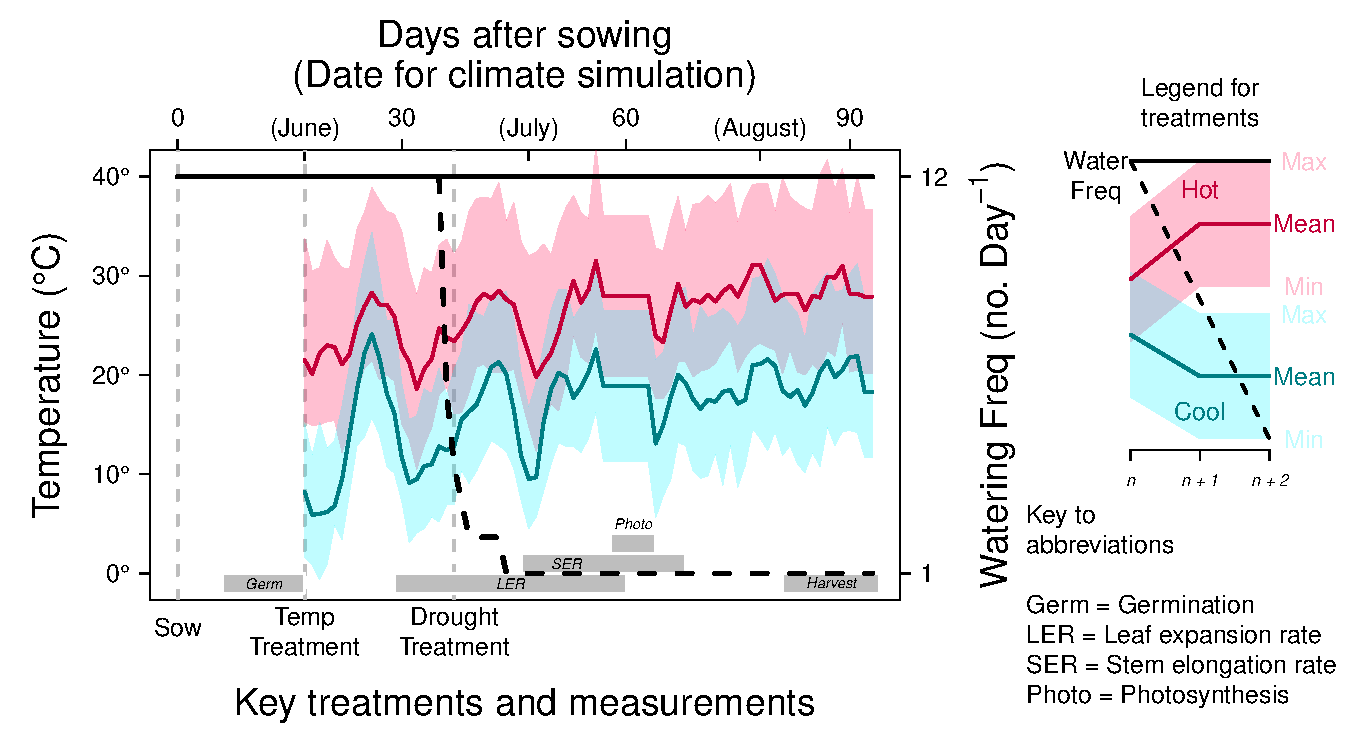
\includegraphics[width=1\textwidth]{Figures/Figure_ExptlDes.pdf}}
	\usefont{T1}{phv}{m}{n}
	\fontsize{10}{12}
	\selectfont
	\caption[Experimental Design]{Overview of experimental treatments and timing of key trait measurements. All plants germinated within 21 days of sowing. At that time, we began temperature treatments (left axis), simulating a typical June-August weather pattern at Hot (red) and Cool (blue) sites. The bold lines track the average daily temperatures. Within each day, there was a maximum daytime temperture (top of translucent polygons) and minimum nighttime temperature (bottom of translucent polygons). The drought treatment commenced later by ramping down the frequency of bottom-watering episodes (black line; right axis). Grey boxes on the bottom of the plot outline the period of key measurements described in the Material and Methods.}
	\label{fig:Fig_ExptlDes}
\end{figure}

\subsection*{Growth and photosynthesis}

%%%%%%%%%%%%%%%%%%%%%%%%%%%%%%%%%%%%%%%%%%%%%%%%%%%%%%%%%%%%%%%%%%%%%%%%%%%%%%%%
% Table of key traits
%%%%%%%%%%%%%%%%%%%%%%%%%%%%%%%%%%%%%%%%%%%%%%%%%%%%%%%%%%%%%%%%%%%%%%%%%%%%%%%%

\begin{table}[ht]
   \centering
   \topcaption{Key traits measured in this study.}
   \begin{tabular}{@{} ll @{}}
      \toprule
  Trait & Units \\
      \midrule
  Days to germination  & day \\
  Leaf expansion rate  &  mm day$^{-1}$  \\
  Stem elongation rate  &  mm or cm day$^{-1}$  \\
  Photosynthetic rate &  $\mu$mol CO$_2$ m$^{-2}$ s$^{-1}$\\
  Mortality & probability of death  \\
	    \bottomrule
   \end{tabular}
   \label{table:Table_traits}
\end{table}

\paragraph{Days to germination} We tested for population variation in germination rate, measured as Days to Germination, using a lognormal survival model fit using the survreg function in the R package \pkg{survival} version 2.38 \citep{Therneau_2015}. We treated Population as a fixed effect and Family as random effect using a $\Gamma$ frailty function. Statistical signifcance of the Population effect was determined using analysis of deviance. Note that, unlike other traits discussed below, we did not include Block, Treatment, or Population $\times$ Treatment interactions because during germination plants had not been placed into blocks and treatments had not yet been applied.


\paragraph{Growth rate: leaf expansion and stem elongation}

We measured growth rate during two phases: leaf expansion as a rosette and stem elongation after bolting. We censused leaf length twice per week from 12 May -- 12 June (28--59 days after sowing), resulting in 10 measurements. We ceased measuring leaf length once it appeared to asymptote and growth shifted to stem elongation.  We also censused plant height on 7 occasions (twice per week) between 29 May and 20 June (45 to 67 days after sowing). Both leaf expansion and stem elongation were modeled as second-order polynomials of time with individual coefficients (separate for leaf and stem growth) using empirical Bayes' estimates from linear mixed-effects models fit with the R package \pkg{lme4} version 1.1-12 \citep{Bates_etal_2015}.




\paragraph{Photosynthesis}
During the week of 10 to 16 June (57 to 63 days after sowing), we measured daytime photosynthetic rate on a subset of 329 plants evenly spread between treatments and families within populations. The youngest, fully-expanded leaf acclimated for 3 minutes to reach steady state in a 6-cm$^2$ chamber of a LI-COR 6400XT Portable Photosynthesis System (LI-COR Biosciences, Lincoln, Nebraska). We made all measurements at ambient light (400 $\mu$mol m$^{-2}$ s$^{-1}$ of photosynthetically active radiation), atmospheric CO$_2$ (400 ppm), temperature, and moderate relative humidity. During this period, we suspended normal day-to-day temperature fluctuations and set daytime temperatures to its average for that period (Cool: 26.5$\degree$; Hot: 36.1$\degree$ so that all plants within a temperature level could be measured under the same conditions. % As expected, stomatal conductance was strongly correlated with photosynthetic rate (results not shown), but we found that treatment and population effects were more apparent when stomatal conductance was factored out. Therefore, we calculated the `intrinsic' photosynthetic rate for each individual as its residual deviance from the regression between stomoatal conductance and photosynthetic rate across all plants. We also removed one outlier.


\paragraph{Mortality}
We assayed mortality during twice-weekly growth measurements. We analyzed the probability of surviving until the end of the experiment as a function of population, treatment, and their interactions using a Generalized Linear Mixed Model (GLMM) assuming binomially distributed errors. We included Family and Block as random effects. We assessed significance of fixed effects using Type-II Analysis of Deviance with Wald $\chi ^2$ tests in the R package \pkg{car} \citep{Fox_Weisberg_2011}. 


\subsection*{Intrinsic variation and plasticity}

For all traits (Table~\ref{table:Table_traits}) except germination (see above), we tested for Population, Treatment, and Population $\times$ Treatment interactions. We interpreted significant Population effects to indicate intrinsic variation and Population $\times$ Treatment interactions to indicate variation in plasticity. As mentioned above, we used survival and GLMM models for germination rate and mortality, respectively. For all other traits, we used mixed model ANOVAs with Family and Block included as random factors. We fit models using restricted maximum likelihood in lmer, a function in the R package \pkg{lme4} \citep{Bates_etal_2015}. We determined significant fixed effect terms using a step-wise backward elimination procedure implemented with the step function in the R package \pkg{lmerTest} version 2.0-32 \citep{Kuznetsova_etal_2016}. This package uses Satterthwaite's approximation to calculate denominator degrees of freedom for $F$-tests. We also included days to germination as a covariate in growth analyses. % To ensure that Population and Treatment effects were specific to a particular growth phase, we included earlier growth phases as a covariate. Specifically, we included germination day as a covariate in leaf expansion and stem elongation analyses; we included germination day and leaf expansion rate as a covariate in stem elongation analyses. 

\subsection*{Principal components of germination, growth, and photosynthesis}
For each single-trait model above, we extracted the Population coefficient (factoring out Treatment and other effects). The multivariate distribution of these coefficients was then summarized using principal components analysis (PCA). The first principal component of these traits (TraitPC1) loaded positively with germination, growth, and photostynthetic rate, therefore we define this as a phenotypic axis dilineating fast to slow growth.



\subsection*{Identifying putative selective agents}

We found that a population's position along TraitPC1 correlated strongly with the latitude or origin (see Results) and next used Random Forest regression \citep{Liaw_Wiener_2002} to identify putative climatic factors underlying trait-latitude associations in \textit{M. cardinalis}. Hypothesis 1: if a single climatic factor explained more trait variation than latitude alone, this would suggest that that factor is a selective agent underlying the latitudinal cline in our 16 focal populations. Hypothesis 2: if multiple climatic factors together explained trait variation,  we interpreted this as evidence that multiple climatic factors together have generated the latitudinal cline. We hereafter refer to factors identified in this analysis as `Climate-TraitPC1' variables. In addition, to help eliminate potentially spurious correlations between TraitPC1 and climate, we tested for overlap between climatic variables that best predict latitude of all \textit{M. cardinalis} occurrence records, not just the 16 focial populations. We refer to these climatic factors as `Climate-Latitude' variables. The logic is that climatic factors associated with both TraitPC1 and latitude for all populations are more likely to be important selective agents than climatic factors that happen to correlate with TraitPC1 but do not covary with latitude throughout the \textit{M. cardinalis} range. We selected Climate-Latitude and Climate-TraitPC1 variables independently with Variable Selection Using Random Forest (VSURF) algorithm in the R package \pkg{VSURF} version 1.0.3 \citep{Genuer_etal_2016}. VSURF ranks variables by their importance over regression trees in the forest. We kept only variables selected for prediction, the most stringent criterion.

% This is now stated above.
%If latitude is strongly correlated with one or two climatic variables that are responsible for the cline, then there should be one or two climatic variables that are identified in both the Climate-Latitude and Climate-TraitPC1 analyses \ala{and the correlation magnitudes should be high? maybe this language is not technically correct (variable importance more accurate?) but the point is that this prediction needs something about count and the strength}. If latitude is correlated with several climatic agents of selection that are individually weak, but add up to a strong latitudinal cline, then several climatic variables should be weakly correlated \ala{fix this to mirror prior}.

To test the third hypothesis about climatic neighborhoods driving selection, we repeated the same procedure to identify Climate-TraitPC1 variables as above, except that we used spatially averaged climate variables. We sampled climate at 1000 random points (at 90-m resolution) within a 62-km buffer around the 16 focal populations. We chose this buffer size because neutral genetic differentiation increases slowly with geographic distance, indicating significant gene flow between nearby populations \citep{Paul_etal_2016}. Significant spatial autocorrelation persisted for approximately 62 km. Since \textit{M. cardinalis} is found exclusively in riparian areas, we only selected points along streams using the National Hydrogeoraphy Dataset \citep{NHD}. Climatic means and CVs were weighted by their climatic suitability as determined using a multimodel ensemble average of ecological niche models \citep{Angert_ENM}. We distinguish between analyses where climate is inferred from a single point (`point estimated Climate-TraitPC1') versus averaged across a 62-km climatic neighborhood (`spatially averaged Climate-TraitPC1'). 


For Climate-Latitude analyses, we compiled a representative set of 356 recent (since 2000) known \textit{M. cardinalis} occurences. These occurences were thinned by 50\% to correct for uneven sampling from a comprehensive set of herbarium records and an exhaustive field survey in 2010-11 \citep{Angert_ENM}. For both Climate-TraitPC1 analyses (16 focal populations) and Climate-Latitude (many populations), we used a 90-m digital elevation model from HydroSHEDS \citep{Lehner_etal_2006} to extract elevation. Monthly interpolated climate layers were calculated using ClimateWNA version 5.30 \citep{Wang_etal_2012}, which accurately downscales climate data specifically for the rugged topography of western North America. For each occurence, we calculated bioclimatic variables using the biovars function in the R package \pkg{dismo} version 1.1-1 \citep{Hijmans_etal_2016}. In total, we included 24 climate variables, 9 from ClimateWNA and 15 bioclimatic variables (Table~\ref{table:TableS_ClimVars}). The bioclimatic variables included all permutations of two climatic factors, temperature and precipitation, and six temporal scales (annual average, coldest quarter, warmest quarter, wettest quarter, driest quarter, or seasonality) as well as mean diurnal range, isothermality, annual temperature range. For each variable, we calculated both a 30-year normal by averging annual values between 1981 and 2010 and 30-year coefficient of variation, a standardized metric of interannual climatic variation. Temperatures were converted to Kelvin to be on a ratio scale appropriate for calculating the coefficient of variation. 

%--------------------------------------------------
% Results
%--------------------------------------------------

\section*{Results}

\subsection*{A coordinated latitudinal cline in germination, growth, and photosynthesis}

There are strong genetically-based trait differences in time to germination, growth, and photosynthetic rate among populations of \textit{M. cardinalis}, as evidenced by large and significant population effects for these traits (Table~\ref{table:Table_AnovaSummary}). A single principal component captured 71.6 \% of the trait variation among populations, defining an axis of variation from fast to slow growth (Fig~\ref{fig:Fig_PC1vLat}). As we explain below, intrinsic differences between populations in terms of plant function (photosynthesis) and performance (growth) contrasted with the low amount of variation in plasticity. There were similar latitudinal clines for individual traits underlying PC1 (Fig S1-S4).

%%%%%%%%%%%%%%%%%%%%%%%%%%%%%%%%%%%%%%%%%%%%%%%%%%%%%%%%%%%%%%%%%%%%%%%%%%%%%%%%
% Table of Population, Treatment, Population x Treatment interactions
%%%%%%%%%%%%%%%%%%%%%%%%%%%%%%%%%%%%%%%%%%%%%%%%%%%%%%%%%%%%%%%%%%%%%%%%%%%%%%%%

% *** Commented out results from Intrinsic Photosynthetic rate *** %

\begin{table}[ht]
   \centering
   \topcaption[ANOVA summary]{Summary of Population, Treatment, and Population $\times$ Treatment effects. We used different statistical modeling for the diverse traits assayed -- glmer: generalized linear mixed model using the R package \pkg{lme4} \citep{Bates_etal_2015}; lmer: linear mixed model using the R package \pkg{lme4} \citep{Bates_etal_2015}; survreg: survival regression using the R package \pkg{survival} \citep{Therneau_2015}. Note that temperature and water treatments were imposed after germination, hence are not applicable to this trait. Complete analysis of variance/deviance tables for each trait are available in the Supporting Information. Key to statistical significance: *$P < 0.05$; ** $P < 0.01$; *** $P < 0.001$}
   \resizebox{6.5in}{!}{
   \begin{tabular}{@{} lllllll @{}}
      \toprule
    {\raggedleft Trait}                          & Germination & Leaf expansion & Stem elongation & Photosynthesis & Mortality \\
    Statistical model              & survreg     & lmer           & lmer            & lmer           & glmer \\
      \midrule
  Population                       &
    ***  &
    *** &
    *** &
    *** & 
     & \\
  Temperature                      &
    NA                                                          &
    ***    &
    *** &
    ** & 
    *** & \\
  Water                            &
    NA                                                          &
    *   &
       &
     & 
    *** & \\
  Pop $\times$ Temp                &
    NA                                                          &
     &
     &
    * & 
     & \\
  Pop $\times$ Water               &
     NA                                                          &
    * &
     &
     & 
     & \\
  Temp $\times$ Water              &
    NA                                                          &
     &
     &
     & 
    *** & \\
  Pop $\times$ Temp $\times$ Water &
    NA                                                          &
     &
     &
     & 
     & \\
      \bottomrule
   \end{tabular} }
   \label{table:Table_AnovaSummary}
\end{table}

%%%%%%%%%%%%%%%%%%%%%%%%%%%%%%%%%%%%%%%%%%%%%%%%%%%%%%%%%%%%%%%%%%%%%%%%%%%%%%%%
% Figure of latitude versus PC1 (growth axis)
%%%%%%%%%%%%%%%%%%%%%%%%%%%%%%%%%%%%%%%%%%%%%%%%%%%%%%%%%%%%%%%%%%%%%%%%%%%%%%%%

\begin{figure}[h!]
	\centerline{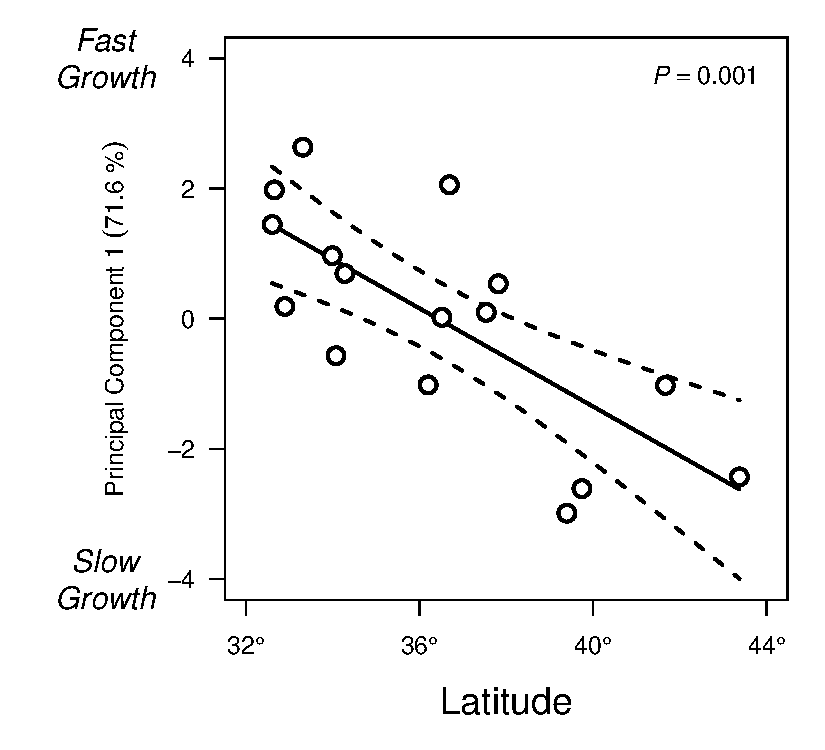
\includegraphics[width=1\textwidth]{Figures/Figure_PC1vLat.pdf}}
	\usefont{T1}{phv}{m}{n}
	\fontsize{10}{12}
	\selectfont
	\caption[Southern populations grow faster]{Trait variation, from fast to slow growth, is closely associated with latitude. Each point is a population's latitude of origin (x-axis) and position along the slow to fast growth axis (y-axis), defined as Principal Component 1 of four traits (see Material and Methods). The line and 95\% confidence intervals were estimated using linear regression.}
	\label{fig:Fig_PC1vLat}
\end{figure}

\subsection*{Little evidence for variation in plasticity}

Genotype $\times$ environment (G$\times$E) interactions are also a common signature of local adaptation. We found little evidence G$\times$E in \textit{M. cardinalis}. There were only two statistically significant Population $\times$ Treatment interaction (Table~\ref{table:Table_AnovaSummary}), but these were not strong compared to Population and Temperature effects. Otherwise, populations responded similarly to treatments: faster growth in the hot treatment, slower growth in the dry treatment, and high mortality in the hot, dry treatment (Table~\ref{table:Table_AnovaSummary}). Note that interactions were calculated after factoring out intrinsic trait differences, necessarily reducing statistical power to detect significant interactions relative to main effects. However, the fact that the Population and Treatment effects were often highly significant ($P \ll 0.001$ in most cases) suggests that statistical power alone cannot explain why we failed to detect Population $\times$ Treatment interactions. Complete ANOVA tables are available in the Supporting Information (Table S3-S6).

\subsection*{Climatic variability best explains latitudinal cline}

Latitudinal clines are common, but it is often difficult to ascribe this variation to a particular selective agent. For \textit{M. cardinalis}, interannual variation in precipitation over 30 years (1981--2010) is very closely related to the latitude of recently recorded occurences of this species (Fig.~\ref{fig:Fig_ClimVarImp}A). Specifically, precipitation is more variable at lower latitude. The two most important Climate-Latitude variables were the interannual variation in total precipitation (bio12$_\sigma$; see Table.~\ref{table:TableS_ClimVars} for a key to climate variable abbreviations) and precipitation in the wettest quarter (bio16$_\sigma$). Note that the coefficient of variation of a climatic factor is subscripted with $\sigma$ whereas the mean is subscripted with $\mu$. Bio12$_\sigma$ and bio16$_\sigma$ are very similar because in Mediterranean climates of California, most precipitation occurs in the winter quarter. These Climate-Latitude variables were also the two most important point estimated Climate-TraitPC1 variables (Fig.~\ref{fig:Fig_ClimVarImp}B). Populations from Southern, more variable environments grew faster. However, neither climatic variable alone explained more variation in TraitPC1 than latitude (latitude $r^2=0.55$; bio16$_\sigma$ $r^2=0.52$; bio12$_\sigma$ $r^2=0.47$). Interannual variation in chilling degree-days (DD\_0$_\sigma$) was also common to both Climate-Latitude and Climate-TraitPC1 analyses (Fig.~\ref{fig:Fig_ClimVarImp}). Southern, faster growing populations are from climates with less variation in chilling degree-days. However, DD\_0$_\sigma$ and bio16$_\sigma$ together still only explained slightly more variation in TraitPC1 than latitude alone (latitude $r^2=0.55$ versus DD\_0$_\sigma$+bio16$_\sigma$ $r^2=0.6$). This suggests that interannual variation in precipitation explains most of the latitudinal cline, but other variables such as variation in chilling degree-days may contribute.

There was no overlap between Climate-Latitude and spatially averaged Climate-TraitPC1 (Fig.~\ref{table:TableS_ClimVarImp}). This is not because climatic neighboorhood did not predict TraitPC1; there were significant correlations between important spatially averaged climatic factors and TraitPC1 that explained as much variation as latitude (data not shown). If these correlations are spurious, this indicates that climatic neighborhood is not as imporant as climate in the immediate vicinity of a population. Conversely, the climatic neighborhood may be important among our focal populations and depart from rangewide correlations between latitude and climate. Since these analyses are exploratory and prone to overinterpretation, we believe the closer overlap between Climate-Latitude and point estimated Climate-TraitPC1 variables provides more compelling evidence for putative selective agents.

%%%%%%%%%%%%%%%%%%%%%%%%%%%%%%%%%%%%%%%%%%%%%%%%%%%%%%%%%%%%%%%%%%%%%%%%%%%%%%%%
% Figure of climatic variable importance
%%%%%%%%%%%%%%%%%%%%%%%%%%%%%%%%%%%%%%%%%%%%%%%%%%%%%%%%%%%%%%%%%%%%%%%%%%%%%%%%

\begin{figure}[h!]
	\centerline{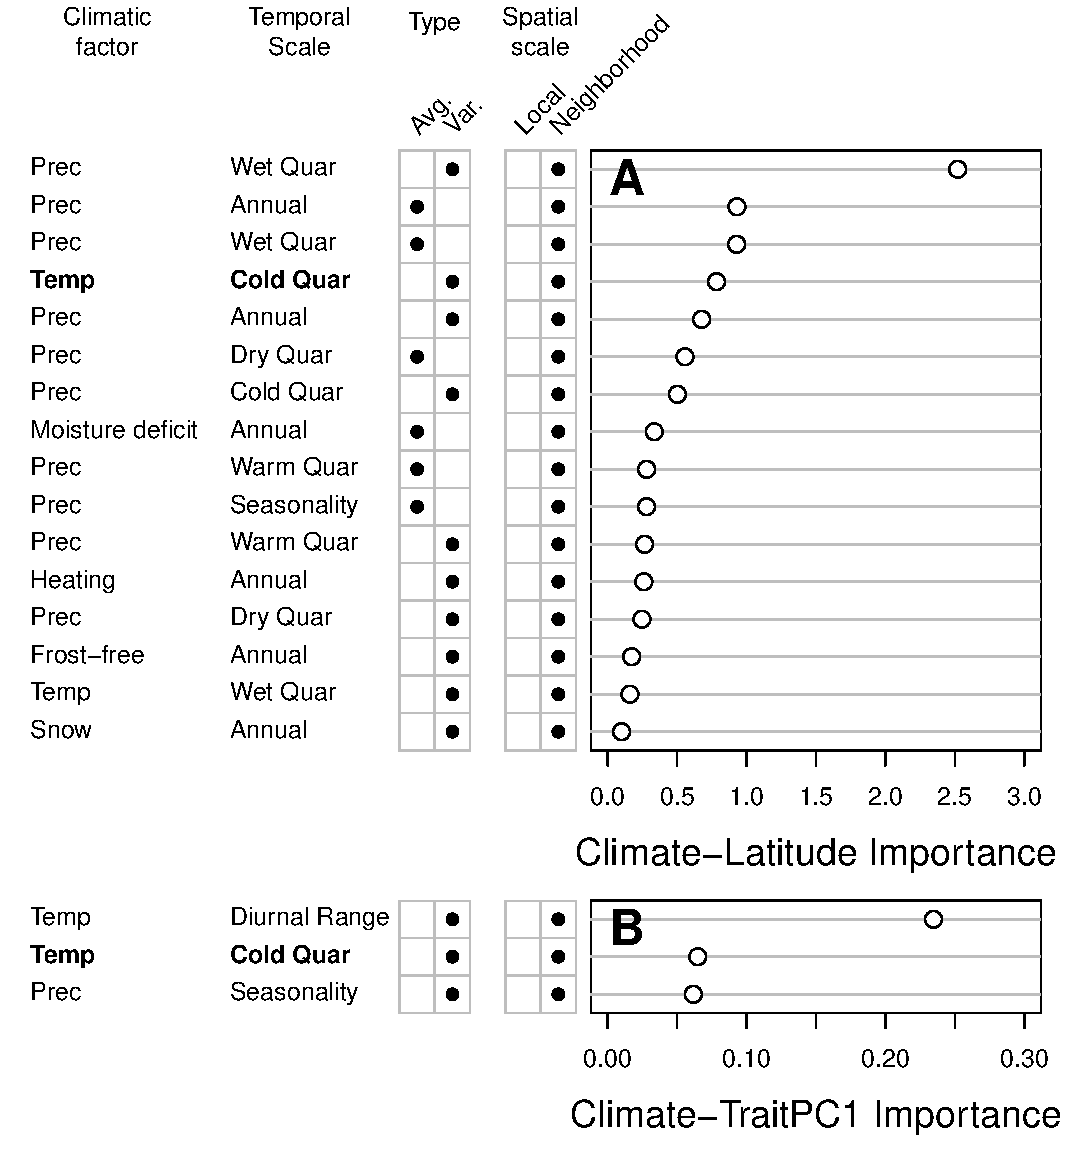
\includegraphics[width=1\textwidth]{Figures/Figure_ClimVarImp.pdf}}
	\usefont{T1}{phv}{m}{n}
	\fontsize{10}{12}
	\selectfont
	\caption[Interannual variation in precipitation is closely correlated with latitude and trait variation]{Interannual variation in precipitation is closely correlated with latitude and trait variation. A. Using Random Forest regression, we identified 11 climatic variables significantly (high importance) associated with latitude of \textit{M. cardinalis} occurences. B. The two most important Climate-Latitude variables were also the two most important Climate-TraitPC1 variables. Note that the Importance values in A and B are not comparable because the dependent variables (Latitude and Trait PC1, respectively) are on different scales. Climatic variables (left of A; right of B) are defined by three qualities: Climatic factor -- Temperature (Temp), Precipitation (Prec), Chilling (chilling degree-days), Snow (precipitation as snow); Temporal scale -- Annual, Coldest quarter (Cold Quar), Warmest Quarter (Warm Quar), Wettest quarter (Wet Quar), Driest Quarter (Dry Quar), or Seasonality; Summary statistic -- average ($\mu$) or coefficient of variation ($\sigma$)}
	\label{fig:Fig_ClimVarImp}
\end{figure}

%--------------------------------------------------
% Discussion
%--------------------------------------------------

% Maybe focus in on tradeoffs as sine qua non of specialization vs generalization, then mention that demography and/or gene flow could reinforce?

% perhaps responses of Simiolus sp (annual, drought selects for escape rather than tolerance) differ from card (perennial, escape through growth rather than flowering time) because drying out of rivers is less severe than seeps and springs?

\section*{Discussion}

% From Amy: \ala{the results that underlie this statement [niche conservation] need more emphasis in the methods}
We found evidence for one of two common signatures of local adaptation in the perennial herb \textit{Mimulus cardinalis}. Latitudinal clines in germination rate, photosynthesis, and growth, suggests adaptive differentiation in fundamental physiological traits of the species. However, we found little evidence that populations respond differently to temperature or drought. As we discuss below, this may indicate that the fundamental abiotic niche is relatively conserved. Finally, we found that climatic variation between years may be a more important selective agent than the average climate. In the paragraphs that follow, we tie these results into the broader threads of evolutionary theory that might help explain why intrinsic variation in photosynthesis and growth varies clinally, but plastic responses to temperature and drought are relatively conserved.

Evolutionary theory indicates that the shape of fitness tradeoffs, demography, and gene flow can constrain adaptation \citep{Levins_1968, Ronce_Kirkpatrick_2001} and hence the type of variation maintained within species. Specifically, adaptive variation cannot be maintained by spatially varying selection if tradeoffs are too strong, demography is strongly asymmetric, and/or maladaptive gene flow is too high. In \textit{M. cardinalis} we found substantial genetically based variation among populations along a phenotypic axis from fast to slow growth that varied over a large spatial scale (Fig.~\ref{fig:Fig_PC1vLat}). If this variation is adaptive, it suggests that the fitness tradeoff between doing well in low versus high latitude environments is not too strong nor swamped by demographic asymmetry or maladaptive gene flow. That is, alleles favoured at one latitude are not strongly selected against when they flow to another population, allowing locally adaptive genetic variation to be maintained by spatially heterogenous selection. We also know from previous work that population size does not vary strongly with latitude. Gene flow appears to be high, but attenuates at broad spatial scales, especially between Southern ($<35\degree$N) and Northern portions of the range \citep{Paul_etal_2016}. 

Another possibility we could have seen is that southern populations, which appear to experience more frequent drought years (see next section), could have evolved the ability to tolerate drought better than northern populations, thereby expanding the fundamental niche of the species as a whole. We found no evidence for this; all populations responded to drought and temperature similarly (Table~\ref{table:Table_AnovaSummary}). Plants grew faster in the Hot treatment, but there was little effect of drought on growth. Rather, the effects of drought took longer to materialize but resulted in high mortality, especially in the Hot chamber. However, there was no differential mortality among populations in this treatment. We hypothesize that evolution of the fundamental niche may be constrained by a combination of strong fitness tradeoffs, demographic asymmetry, and gene flow. Riparian habitats where \textit{M. cardinalis} live are highly heterogeneous at small spatial scales. Plants in the stream never have to tolerate drought whereas plants only a few meters away may experience extreme drought since there is little direct precipitation during the growing season in Mediterranean climates of western North America. But alleles that confer greater drought tolerance may be quite costly in well-watered soils, and vice versa, leading to strong fitness tradeoffs. Such tradeoffs promote specialization to one soil type or another, thereby inhibiting the evolution of broad environmental tolerance within a population. Demography and gene flow may reinforce niche conservatism. A new mutant with increased drought tolerance that can survive at the resource-poor margin of a population will be demographically overwhelmed by the larger census populations that can be maintained in higher resource environments. Infrequent wet years may also produce most seeds, so selection weighted towards wet environment even if dry years are more frequent. Finally, gene flow, which is generally high among \textit{M. cardinalis} populations within the same ecoregion \citep{Paul_etal_2016}, will thwart local adaptation and reinforce specialization. Thus, the spatial grain of the environment, demographic asymmetry, and gene flow may conspire to constrain local adaptation via altered fundamental niche.

Based on the available data, interannual variation in annual or winter precipitation (these are closely correlated in Mediterranean climates) may be the selective agent driving variation in physiological traits. Variation in precipitation was best predicted latitude of recent \textit{M. cardinalis} occurences and trait variation along the fast-slow growth continuum (Fig.~\ref{fig:Fig_ClimVarImp}). A life history tradeoff between allocation to growth in the current year at the expense of future years could explain this pattern. In southern populations with more frequent droughts capable of killing rhizomes, a more annualized strategy could be favored. Conversely, in more predictable northern environments, lifetime fitness may be optimized when a significant fraction of assimilate is allocated below ground for future years. Although this hypothesis remains to be directly tested, a few independent lines of evidence are consistent with it. Preliminary surveys suggest that northern populations not only grow slower, but also produce greater numbers of rhizomes (C.D. Muir, unpub. data), suggesting an allocation tradeoff. Ecological niche models also show that occurence of southern populations is best predicted by recent climate (< 5 years), whereas northern occurences are best predicted by climate over the previous 30 years (M. Bayly \& A. Angert, unpub. data). Finally, demographic surveys of natural populations show greater variation in the size of recruits in southern populations, suggesting higher maximum growth rates under natural conditions (M. Bayly \& A. Angert, unpub. data). There is a lot of interest in understanding how organisms will respond to changes in climatic variation, not just changes in the average climate. Our data indeed suggest that variation may be more important than the mean. 

In summary, we found evidence for a coordinated latitudinal cline in germination rate, photosynthesis, and growth, suggesting local adaptation. These fixed differences between populations suggest different trait optima in different climates. We did not find evidence that the relative performance of populations shifts with temperature or watering regime, suggesting relatively little variation in plasticity. Exploratory analysis implicate that more variable precipitation regimes at lower latitude drive much of the latitudinal cline, though other climatic factors could also contribute. There was little compelling evidence that selection over a broad climatic neighborhood surrounding populations strongly explained the latitudinal cline. In the future, we will use field experiments to test whether greater variation in precipitation selects for faster growth and that selection on temperature/drought responses does not vary among populations. By doing so, we aim to understand why certain physiological and developmental mechanisms, but not others, contribute to local adaptation.

% [Future work and broad conclusions]. Supports general conclusions that traits related to timing and growth are evolutionarily labile whereas those related to the fundamental niche are constrained (cites like \cite{Emery_etal_2012, Emery_Ackerly_2014}). Next, we are testing whether phenotypic variation and constraint can be predicted by the shape of tradeoffs, as predicted by evolutionary theory. \cdm{I will work more on this once I am more comfortable with the rest of the discussion}.

% niche-tracking versus niche-shifting
% One surprising pattern is that populations adapt to different environments by adjusting their life history to stay within the same fundamental physiological niche rather than have the niche itself evolve. For example, mosquitoes adjust diapause length with latitude rather than evolve altered ...\cdm{what other examples could we include here?} This suggests that in many situations it is evolutionarily easier to change life history rather than fundamental physiological tolerance.




% citations on life history allocation tradeoff between growth and reproduction:
%% THEORY:
% Bell 1980 - briefly mentionds on page 56 that increased environmental variation for adults will favor semelparity
% Iwasa and Cohen 1989, pg. 496 "A larger reliability of habitat, a higher storage efficiency, higher productivity of the environment, and a longer growing season, all tend to promote the evolution of perennial life, as suggested by previous models of life-historsy strategy (Stearns 1976).

%% EMPIRICAL:
% Sawada et al. 1994 - latitudinal cline dry matter accumulation and storage allocation
% Stanton et al 2000 show selection in stressful environemts (artificual selection over 5 generations) favors stress avoidance rather than tolerance traits. i.e. might be easier to adjust life history rather than tolerance.
% Hall and Willis 2006 find selection on flowering time in coastal-inland comparison of M guttatus
% Ehleringer et al 1990 find lower WUE increased yield in ephemeral pops
% Bazzaz 1979: higher photo in fast growing plants (early succession)

% Reznick 1985; Lovett Doust 1989
% Williams 1966; Charnov and Schaffer 1973; Bell 1980; Reznick 1985; Biere 1995; Johnson 2007).
% for iteroparous sp: van Noordwijk and De Jong 1986.
% from Remington et al. 2013: "Genetic variation in traits subject to trade-offs results in what has been termed “structured pleiotropy,” in which genetic covariances between traits result from functional constraints imposed by the limiting resources (De Jong 1990; Stearns et al. 1991; see Figure 1B).


%--------------------------------------------------
% Acknowledgements
%--------------------------------------------------

% *** Need to fill in exact grant numbers *** %
\section*{Acknowledgements}
Erin Warkman and Lisa Lin helped collect data. CDM was supported by a Biodiversity Postdoctoral Fellowship funded by the NSERC CREATE program. ALA was supported by an NSERC Discovery Grant and a grant from the National Science Foundation.

%--------------------------------------------------
% References
%--------------------------------------------------

\setlength{\bibsep}{6pt}
\bigskip

\bibliography{../../CommonResources/refs}
\bibliographystyle{evolution}

\clearpage

%--------------------------------------------------
% Supporting Information
%--------------------------------------------------

\section*{Supporting Information}

% Modify and restart table/figure numbering for appendixes
\renewcommand\thefigure{S\arabic{figure}}    
\renewcommand\thetable{S\arabic{table}}    
\renewcommand\theequation{S\arabic{equation}}    
\setcounter{table}{0}    
\setcounter{equation}{0}
\setcounter{figure}{0}

%--------------------------------------------------
% Supporting Tables
%--------------------------------------------------

\subsection*{Supporting Tables}

% DIC table for initial size (LLL on 5/12)
\begin{table}[htbp]
	\usefont{T1}{phv}{m}{n}
	\fontsize{10}{12}
	\selectfont
	\caption[DIC table for initial size of seedlings]{Initial size of seedlings did not vary among Populations, Families, or Treatments. We used a censored Gaussian model of initial size at the outset of the experiment (longest leaf length of the first true leaves). The model was censored because we could not accurately measure leaves less than 0.25 mm with digital callipers (217 of 702, 30.9\%, were too small). We fit models using a Bayesian MCMC method implemented using the MCMCglmm function with default priors in the R package \pkg{MCMCglmm} version 2.17 \citep{Hadfield_2010}. We estimated the posterior distribution from 1000 samples of an MCMC chain run for $10 ^ 5$ steps after a $10^4$ step burn-in. We used step-wise backward elimination procedure to find the best-supported model according to Deviance Information Criterion (DIC).}
	\begin{center}
	\begin{tabular}{>{\everypar{\hangindent1cm}{}\raggedright}p{6cm}lc}
	\toprule

	\input{Tables/Table_InitialSize.txt}

	\bottomrule
	\end{tabular}
	\end{center}
	\label{table:TableS_InitialSize}
\end{table}

\begin{table}[ht]
	\caption[Climate variables]{Climatic variables used }
   \centering
   \begin{tabular}{@{} ll @{}}
      \toprule
   Abbreviation & Climate variable \\
      \midrule
  % climateWNA VARIABLES:
	DD\_0	& degree-days below 0\celsius (chilling degree-days)  \\
	DD5	  & degree-days above 5\celsius (growing degree-days)   \\
	DD\_18	& degree-days below 18\celsius (heating degree-days)  \\
	DD18	& degree-days above 18\celsius (cooling degree-days)  \\
	NFFD	& number of frost-free days                           \\
	PAS	  & precipitation as snow (mm) between August in previous year and July in current  \\
	Eref	& Hargreaves reference evaporation (mm) \\
	CMD	  & Hargreaves climatic moisture deficit (mm) \\
	RH    &	mean annual relative humidity \\
  % BIOCLIM VARIABLES:
  bio1	&	Annual Mean Temperature	\\
	bio2	&	Mean Diurnal Range (Mean of monthly (max temp - min temp))	\\
	bio3	&	Isothermality (bio2/bio7) (* 100)	\\
	bio4	&	Temperature Seasonality (standard deviation *100)	\\
	bio5	&	Max Temperature of Warmest Month	\\
	bio6	&	Min Temperature of Coldest Month	\\
	bio7	&	Temperature Annual Range (bio5-bio6)	\\
	bio8	&	Mean Temperature of Wettest Quarter	\\
	bio9	&	Mean Temperature of Driest Quarter	\\
	bio10	&	Mean Temperature of Warmest Quarter	\\
	bio11	&	Mean Temperature of Coldest Quarter	\\
	bio12	&	Annual Precipitation	\\
	bio15	&	Precipitation Seasonality (Coefficient of Variation)	\\
	bio16	&	Precipitation of Wettest Quarter	\\
	bio17	&	Precipitation of Driest Quarter	\\
	bio18	&	Precipitation of Warmest Quarter	\\
	bio19	&	Precipitation of Coldest Quarter	\\
	    \bottomrule
   \end{tabular}
   \label{table:TableS_ClimVars}
\end{table}

% Analysis of deviance table for germination


% *** NEED TO DO TABLE IF I WANT IT ***

% ANOVA table for LER


\begin{table}[htbp]
	\usefont{T1}{phv}{m}{n}
	\fontsize{10}{12}
	\selectfont
	\caption[ANOVA table, leaf expansion rate]{Analysis of varianace (ANOVA) table on leaf expansion rate (LER) using \pkg{lmerTest} \citep{Kuznetsova_etal_2016}. Family and Block were included as random effects. Abbreviations: SS = sum of squares; MS = mean sum of squares (SS / df1); df1 = numerator degrees of freedom; df2 = denominator degrees of freedom.}
	\begin{center}
	\begin{tabular}{lcccccc}
	\toprule

  & SS & MS & df1 & df2 & \em{F}-value & $P$-value \\ \midrule
  Day to Germination & 12.12 & 
    12.12 & 1 & 
    637 & 35.21 &
    4.9 $\times10^{-9}$ \\
  Population & 22.22 & 1.48 & 
    15 & 118 & 
    4.3 & 2.5 $\times10^{-6}$ \\
  Temperature & 80.42 & 
    80.42 & 1 &
    5 & 233.61 &
    2.6 $\times10^{-5}$ \\
  Water & 4.1 & 4.1 & 
    1 & 5 & 
    11.92 & 0.019 \\
  Temperature $\times$ Water & 0.03 & 
    0.03 & 
    1 & 
    4 & 
    0.07 &
    0.801 \\
  Population $\times$ Temperature & 2.76 & 
    0.18 & 
    15 & 
    547 & 
    0.53 &
    0.925 \\
  Population $\times$ Water & 9.66 & 
    0.64 & 
    15 &
    562 &
    1.87 & 
    0.024 \\
  Population $\times$ Temperature $\times$ Water & 
    4.11 & 
    0.27 & 
    15 & 
    530 & 
    0.78 & 
    0.700 \\
	\bottomrule
	\end{tabular}
	\label{table:TableS_fitLER}
	\end{center}
\end{table}

% ANOVA table for SER


\begin{table}[htbp]
	\usefont{T1}{phv}{m}{n}
	\fontsize{10}{12}
	\selectfont
	\caption[ANOVA table, stem elongation rate]{Analysis of varianace (ANOVA) table on stem elongation rate (SER) using \pkg{lmerTest} \citep{Kuznetsova_etal_2016}. Family and Block were included as random effects. Abbreviations: SS = sum of squares; MS = mean sum of squares (SS / df1); df1 = numerator degrees of freedom; df2 = denominator degrees of freedom.}
	\begin{center}
	\begin{tabular}{lcccccc}
	\toprule

  & SS & MS & df1 & df2 & \em{F}-value & $P$-value \\ \midrule
  Day to Germination & 3.6 & 
    3.6 & 1 & 
    662 & 21.1 &
    5.1 $\times10^{-6}$ \\
  Population & 12 & 0.8 & 
    15 & 113 & 
    4.7 & 5.8 $\times10^{-7}$ \\
  Temperature & 12.4 & 
    12.4 & 1 &
    6 & 72.8 &
    1.5 $\times10^{-4}$ \\
  Water & 0.6 & 0.6 & 
    1 & 5 & 
    3.7 & 0.113 \\
  Temperature $\times$ Water & 0.9 & 
    0.9 & 
    1 & 
    4 & 
    5.2 &
    0.093 \\
  Population $\times$ Temperature & 3.6 & 
    0.2 & 
    15 & 
    549 & 
    1.4 &
    0.126 \\
  Population $\times$ Water & 2.8 & 
    0.2 & 
    15 &
    536 &
    1.1 & 
    0.330 \\
  Population $\times$ Temperature $\times$ Water & 
    1.5 & 
    0.1 & 
    15 & 
    518 & 
    0.6 & 
    0.874 \\
	\bottomrule
	\end{tabular}
	\label{table:TableS_fitSER}
	\end{center}
\end{table}

% ANOVA table for photosynthesis


\begin{table}[htbp]
	\usefont{T1}{phv}{m}{n}
	\fontsize{10}{12}
	\selectfont
	\caption[ANOVA table, photosynthesis]{Analysis of varianace (ANOVA) table on photosynthetic rate using \pkg{lmerTest} \citep{Kuznetsova_etal_2016}. Family and Block were included as random effects. Abbreviations: SS = sum of squares; MS = mean sum of squares (SS / df1); df1 = numerator degrees of freedom; df2 = denominator degrees of freedom.}
	\begin{center}
	\begin{tabular}{lcccccc}
	\toprule

  & SS & MS & df1 & df2 & \em{F}-value & $P$-value \\ \midrule
  Population & 347.7 & 
    23.2 & 15 &
    78 & 3.02 &
    7.5 $\times10^{-4}$ \\
  Temperature & 134.1 & 
    134.1 & 1 &
    6 & 17.46 &
    6.4 $\times10^{-3}$ \\
  Water & 51 & 
    51 & 1 &
    4 & 6.64 &
    0.066 \\
  Temperature $\times$ Water & 0.7 & 
    0.7 & 
    1 & 
    3 & 
    0.09 &
    0.781 \\
  Population $\times$ Temperature & 218.6 & 
    14.6 & 
    15 & 
    263 & 
    1.9 &
    0.024 \\
  Population $\times$ Water & 87.7 & 
    5.8 & 
    15 &
    233 &
    0.76 & 
    0.724 \\
  Population $\times$ Temperature $\times$ Water & 
    91.4 & 
    6.1 & 
    15 & 
    208 & 
    0.79 & 
    0.686 \\
	\bottomrule
	\end{tabular}
	\label{table:TableS_fitPhoto}
	\end{center}
\end{table}

% Analysis of deviance table for mortality


\begin{table}[htbp]
	\usefont{T1}{phv}{m}{n}
	\fontsize{10}{12}
	\selectfont
	\caption[Analysis of deviance table, mortality]{Analysis of deviance table on the probability of mortality by the end of the experiment using Type-II Wald $\chi ^2$ tests in the R package \pkg{car} \citep{Fox_Weisberg_2011}. Family and Block were included as random effects. Abbreviations: df = degrees of freedom}
	\begin{center}
	\begin{tabular}{lccc}
	\toprule

  & $\chi ^2$ & df & $P$-value \\ \midrule
  Population & 32 & 
    31 & 0.419 \\
  Temperature & 31.8 & 
    6 & 1.8 $\times10^{-5}$ \\
  Water & 69.2 & 
    12 & 4.6 $\times10^{-10}$ \\
  Temperature $\times$ Water & 20.7 & 
    1 & 
    5.3 $\times10^{-6}$ \\
  Population $\times$ Temperature & 5.6 & 
    15 & 
    0.985 \\
  Population $\times$ Water & 8.6 & 
    15 & 
    0.897 \\
  Population $\times$ Temperature $\times$ Water & 
    0.2 & 
    15 & 
    1.000 \\	\bottomrule
	\end{tabular}
	\label{table:TableS_fitMort}
	\end{center}
\end{table}

% Table of Climate-Latitude and Climate-Trait variables

\begin{table}[ht]
   \centering
   \topcaption[Important climatic variables]{Important climatic variables predicting latitude of \textit{M. cardinalis} populations (`Climate-Latitude') and the first principal component of traits measured in a common garden (`Climate-TraitPC1'). Point estimated climatic variables were measured from the exact location of collection; spatially averaged climatic variables were averaged from a 62-km neighborhood around population (see Material and Methods). Importance and significance were determined using the variable selection using random forests (VSURF) algorithm (see Material and Methods). Climatic variables are described in Table~\ref{table:TableS_ClimVars}. $\mu$ signifies the mean of the climate variables from 1981--2010; $\sigma$ indicates coeffiecient of variation among years. }
   \resizebox{6.5in}{!}{
   \begin{tabular}{@{} lll @{}}
      \toprule
    	Climate-Latitude variables & Climate-TraitPC1 variables & \\
                            	   & Point estimated         & Spatially averaged \\
      \midrule
			\input{Tables/TableS_ClimVarImp.txt}
			\bottomrule
   \end{tabular} }
   \label{table:TableS_ClimVarImp}
\end{table}

\clearpage

%--------------------------------------------------
% Supporting Figures
%--------------------------------------------------

\subsection*{Supporting Figures}

% Figures showing latitudinal clines with specific traits

	
\begin{figure}[h!]
	\centerline{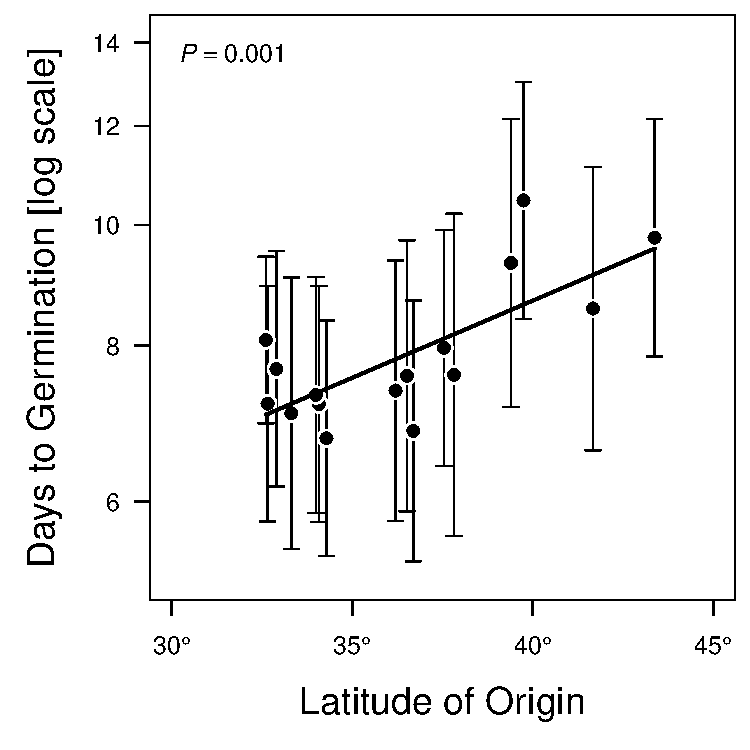
\includegraphics[width=0.5\textwidth]{Figures/FigureS_GermLat.pdf}}
	\usefont{T1}{phv}{m}{n}
	\fontsize{10}{12}
	\selectfont
	\caption[Southern populations germinate faster]{Southern populations germinate faster. Each point is a population of \textit{M. cardinalis} showing its latitude of origin (x-axis) and model-predicted days to germination in days under growth chamber conditions (see Material and Methods). Bars around each point are 95\% confidence intervals. Predicted time to germination and confidence intervals are based on survival regression (see Materials and Materials). The line is the linear regression of log(model-predicated days to germination) $\sim$ latitude. The $P$-value of the regression is given in the upper left corner.}
	\label{fig:FigS_GermLat}
\end{figure}


\begin{figure}[h!]
	\centerline{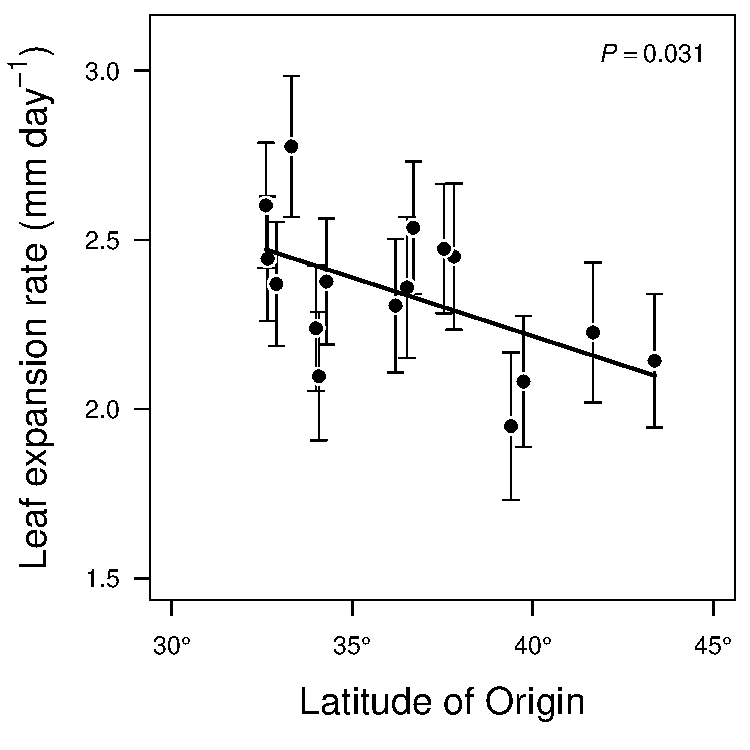
\includegraphics[width=0.5\textwidth]{Figures/FigureS_LERlat.pdf}}
	\usefont{T1}{phv}{m}{n}
	\fontsize{10}{12}
	\selectfont
	\caption[Southern populations grow faster (leaf expansion rate).]{Southern populations grow faster. Each point is a population of \textit{M. cardinalis} showing its latitude of origin (x-axis) and model-predicted leaf expansion rate during the rosette phase. Bars around each point are 95\% confidence intervals. Predicted leaf expansion rate based least-square mean estimates and confidence intervals were calculated from linear mixed-effects models (see Materials and Materials). The line is the linear regression of model-predicated leaf expansion rate $\sim$ latitude. The $P$-value of the regression is given in the upper right corner.}
	\label{fig:FigS_LERlat}
\end{figure}


\begin{figure}[h!]
	\centerline{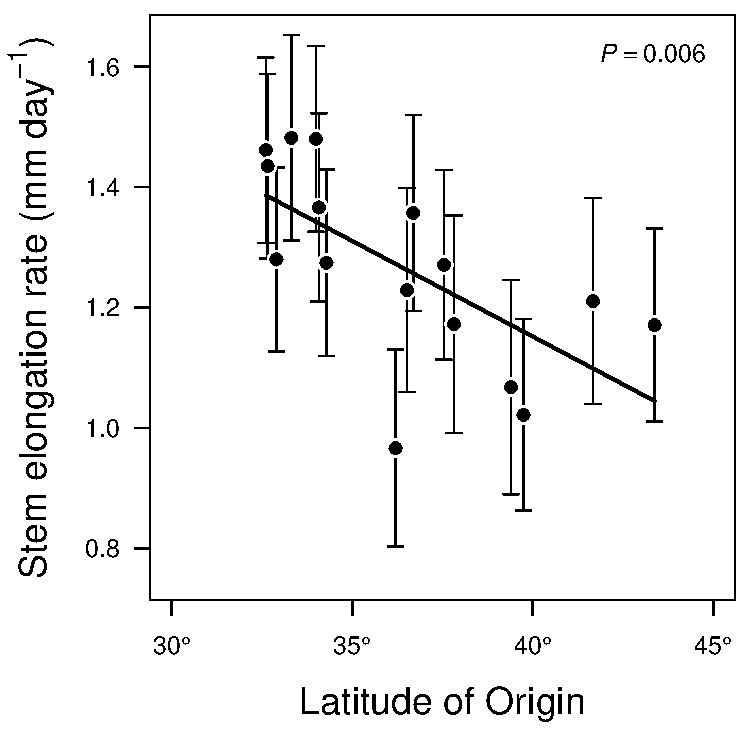
\includegraphics[width=0.5\textwidth]{Figures/FigureS_SERlat.pdf}}
	\usefont{T1}{phv}{m}{n}
	\fontsize{10}{12}
	\selectfont
	\caption[Southern populations grow faster (stem elongation rate).]{Southern populations grow faster. Each point is a population of \textit{M. cardinalis} showing its latitude of origin (x-axis) and model-predicted stem elongation rate during the bolting phase. Bars around each point are 95\% confidence intervals. Predicted stem elongation rate based least-square mean estimates and confidence intervals were calculated from linear mixed-effects models (see Materials and Materials). The line is the linear regression of model-predicated stem elongation rate $\sim$ latitude. The $P$-value of the regression is given in the upper right corner.}
	\label{fig:FigS_SERlat}
\end{figure}


\begin{figure}[h!]
	\centerline{\includegraphics[width=0.5\textwidth]{Figures/FigureS_Photolat.pdf}}
	\usefont{T1}{phv}{m}{n}
	\fontsize{10}{12}
	\selectfont
	\caption[Southern populations photosynthesize faster.]{Southern populations photosynthesize faster. Each point is a population of \textit{M. cardinalis} showing its latitude of origin (x-axis) and model-predicted instantaneous photosynthetic rate. Bars around each point are 95\% confidence intervals. Predicted photosynthetic rates based least-square mean estimates and confidence intervals were calculated from linear mixed-effects models (see Materials and Materials). The line is the linear regression of model-predicated photosynthetic rate $\sim$ latitude. The $P$-value of the regression is given in the upper right corner.}
	\label{fig:FigS_Photolat}
\end{figure}

% Figure comparing importance of climatic variables from point estimated and spatially averaged analyses


% *** Need to double check 62-km buffer results and make figure prettier *** %
% \begin{figure}[h!]
%	\centerline{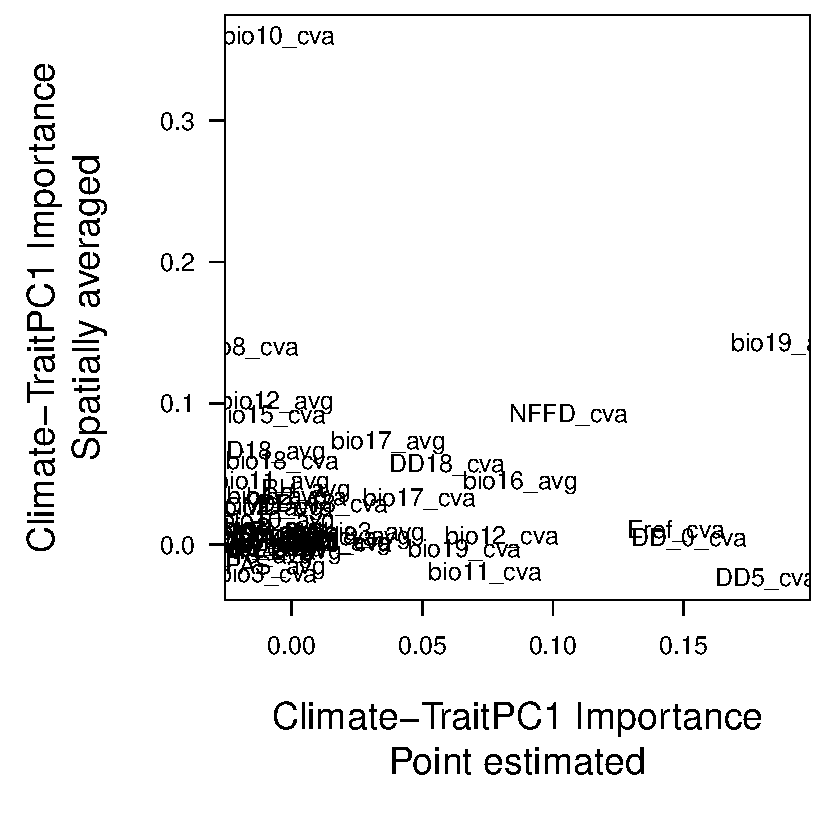
\includegraphics[width=0.5\textwidth]{Figures/FigureS_PEvsSA.pdf}}
%	\usefont{T1}{phv}{m}{n}
%	\fontsize{10}{12}
%	\selectfont
%	\caption[Point-estimated versus spatially averaged importance]{CAPTION}
%	\label{fig:FigS_PEvsSA}
% \end{figure}

\clearpage

\subsection*{Supporting Material and Methods}

\subsubsection*{Temperature treatments}

We simulated typical growing season (June 1 - August 15) air temperatures at the two most thermally divergent focal sites in our study, Whitewater Canyon (WWC, Hot) and Little Jameson (LIJ, Cool). We downloaded daily interpolated mean, minimum, and maximum air temperature from 13 years (2000-2012) at both sites from ClimateWNA \citep{Wang_etal_2012}. This range was chosen because seeds used in the experiment were collected around 2012, thus their presence in that location at that time suggests that populations were able to persist there for at least some years before collection. Monthly temperatures from ClimateWNA are highly correlated with the air temperature recorded from data loggers in the field at these sites (A. Angert, unpub. data). Hence, the ClimateWNA temperature profiles are similar to actual thermal regimes experienced by \textit{M. cardinalis} in nature. We simulated realistic temperature regimes by calculating the mean temperature trend from June to August using LOESS \citep{Cleveland_etal_1992}. The residuals were highly autocorrelated at both sites (warmer than average days are typically followed by more warm days) and there was strong correlation ($r = 0.65$) between sites (warm days in WWC were also warm in LIJ). The `VARselect' function in the \pkg{vars} package for R \citep{Pfaff_2008} indicated that a lag two Vector Autoregression (VAR(2)) model best captured the within-site autocorrelation as well as between-site correlation in residuals. We fit and simulated from the VAR(2) model using the package \pkg{dse} \citep{Gilbert_2014} in R. Simulated data closely resembled the autocorrelation and between-site correlation of the actual data. From simulated mean temperature, we next selected minimum and maximum daily temperatures. Mean, min, and max temperature were highly correlated at both sites. We chose min and max temperatures using site-specific fitted linear models between mean, max, and min temperature, with additional variation given by normally distributed random deviates with variance equal to the residual variance of the linear models. For each day, the nighttime (22:00 - 6:00) chamber temperature was set to the simulated minimum temperature. During the middle of the day, temperature was set to the simulated maximum temperature, with a variable period of transition between min and max so that the average temperature was equal the simulated mean temperature.

\subsubsection*{Watering treatments}

%*** need to check chiller temp and make of chiller
For watering treatments, we simulated two extreme types of streams where \textit{M. cardinalis} grows. In the well-watered treatment, we simulated a large stream that never goes dry during the summer growing season. In the drought treatment, we simulated a small stream that has ample flow at the beginning of the season due to rain and snow melt, but gradually dries down through the summer. In both treatments, plants were bottom-watered using  water chilled to 7.5\celsius. Plants in the well-watered treatment were fully saturated every two hours during the day. Watering in the drought treatment gradually declined from every two hours to every day between May 20 (36 days after sowing) and 10 June (57 days after sowing). Simultaneously, the amount of bottom-watering per flood decreased, such that only the bottom of the cone-tainers were wetted by the end of the experiment.

\end{document}
